\documentclass[12pt,a4paper]{article}

\usepackage{anyfontsize}
\usepackage{graphicx}

%package for list formatting (ordered) if we add [a.]
\usepackage{enumerate}
%package for graphics or include images
\usepackage{graphicx}
\usepackage{float} %to place image forcefully there
\usepackage{pdfpages}
\usepackage{subcaption,caption}
\usepackage[hidelinks]{hyperref}

%for times new roman font
\usepackage{times,mathptmx}


%package for margins
\usepackage[outer=1.25in,inner=1.5in,top=1in,bottom=1in,headheight=0.5in,footskip=0.5in]{geometry}
%better to use outer and inner beacause while printing book then right and left margin will not be good , So, inner margin 


\begin{document}
	\pagenumbering{roman}
	
	
\begin{titlepage}
	
	\newcommand{\HRule}{\rule{\linewidth}{0.3mm}}
	\centering
	\vfill
	
\includegraphics[width=50mm]{images/tu.jpg}\\[0.75cm]
	\textsc{\Large \bfseries  TRIBHUVAN UNIVERSITY}\\[0.25cm] % Name of your university/college
	\textsc{\Large \bfseries INSTITUTE OF ENGINEERING}\\[0.25cm]
	\textsc{\Large \bfseries  PULCHOWK CAMPUS}\\
	\vfill
	\large {A PROJECT PROPOSAL ON }\\
	\Large \textbf{BAAL ARJUN : A 2D ARROW SHOOTING GAME}
	\vfill
	%\large \textbf{Subject code} \\[0.2cm]
%	\bfseries
	\large
	Submitted by:\\
	\textbf{ANUJ SHRESTHA} (078BCT014)\\
	\textbf{ARISHA PRASAIN} (078BCT019)\\
	\textbf{AYUSH ADHIKARI} (078BCT024)\\[0.5cm]
	\vfill
	\large
	A PROJECT PROPOSAL TO THE DEPARTMENT OF ELECTRONICS AND COMPUTER
	ENGINEERING ON OBJECT ORIENTED PROGRAMMING APPLICATION USING
	C++
	\vfill
	SUBMITTED TO:\\
	\textbf{DEPARTMENT OF ELECTRONICS AND COMPUTER ENGINEERING}
	\\
	\vfill
	{\large \today}
	\vfill
\end{titlepage}

	
  	
  	
  	\newpage
\section*{ACKNOWLEDGEMENT}
\addcontentsline{toc}{section}{ACKNOWLEDGEMENT}

We would like to extend our sincere gratitude to our esteemed Lecturer, Mr. Daya Sagar Baral, for granting us the invaluable opportunity to undertake the project work on Object-Oriented Programming in C++. We express our heartfelt appreciation for his invaluable support and guidance, which played a crucial role in ensuring the success of this project. We would also like to express our deepest gratitude to the Department of Electronics and Computer Engineering at the Institute of Engineering, Pulchowk Campus, for providing us with the opportunity to collaborate on this endeavor. Additionally, we extend our thanks to our laboratory instructors for their guidance and support throughout our work in the computer lab.
\\\\
We are immensely thankful to all our friends who have contributed to the development of this project, and we sincerely appreciate their assistance. We welcome constructive criticism and recommendations in any form, and we assure you that they will be received with an open heart, valued, and duly acknowledged.

\vskip 8mm
\begin{flushleft}
	{\bf Authors:}
	\newline Anuj Shrestha
	\newline Arisha Prasain
	\newline Ayush Adhikari		
\end{flushleft}
  %	

\newpage
\section*{ABSTRACT}
\addcontentsline{toc}{section}{ABSTRACT}

The principal aim of this project was to create a gaming program utilizing an Object-Oriented Programming language, C++. Within the scope of this project, we crafted a 2D game centered around arrow-based combat using the Simple and Fast Multimedia Library (SFML) to handle the graphical user interface. The underlying objective of developing this game also encompassed the insights into the world of game development.\\\\
Baal Arjun stands as a 2D, single-player computerized game. This game constitutes a simple two-dimensional rendition of a battlefield, presented from a top-down perspective. In this scenario, the player assumes the role of the character 'Arjuna' and engages in shooting arrows at adversaries and their cohorts. The initial three levels have been designed to function as a means of familiarizing the player with the game interface. Successful completion of each level hinges upon the player's ability to triumph over the adversaries prior to succumbing to their own defeat. Should the player emerge successful in this endeavor, they attain victory; conversely, failure to do so results in defeat.\\\\
\textit{Keywords: Baal Arjun, SFML, Object-Oriented Programming, C++}
  \newpage
  \tableofcontents
  	
%  	\newpage
%  	{
%  		\setlength{\parskip}{0em}
%  		\renewcommand\contentsname{TABLE OF CONTENTS}\\[0.5cm] % This will change heading text
%  		\tableofcontents 
%  	   % \addcontentsline{toc}{section}{TABLE OF CONTENTS}
%  	}
  	
  	
  	
  	\newpage
\pagenumbering{arabic}
\section{OBJECTIVES}
The primary objective of this project is to facilitate the practical application of the Object-Oriented Programming (OOP) model using the well-established and effective programming language, C++. The key objectives pertaining to the development of this project are outlined as follows:

\begin{enumerate}
	\item To gain a comprehensive understanding of the Object-Oriented Programming paradigm, encompassing its principles and successfully implementing them in the project.
	\item To explore the fundamental as well as advanced features offered by C++.
	\item To acquire knowledge and proficiency in designing custom header files, thereby familiarizing ourselves with the concepts of modularity and reusability.
	\item To acquire a foundational understanding of game development and testing, with a specific focus on the development of game.
	\item To become acquainted with graphics libraries such as SFML, enabling the design and implementation of a user-friendly user interface (UI).
	\item To develop a program that exhibits high performance and efficiency, taking the factors such as memory management, time constraints, algorithmic complexity, and optimal resource utilization into consideration. 
	\item To enhance our abilities in teamwork and collaborative communication, fostering effective cooperation among project members.
	
\end{enumerate}

By pursuing these objectives, we aim to gain practical knowledge and skills in OOP principles, C++ programming, modular design, game development practices, UI design, and optimization techniques. Moreover, this project serves as an opportunity to strengthen our collaborative abilities, enhancing our team dynamics and communication skills.

  	\newpage
\pagenumbering{arabic}
\section{INTRODUCTION}
Baal Arjun is a 2D arrow shooting game that takes inspiration from the esteemed character Arjuna in the epic Mahabharata, who is widely regarded as the preeminent archer of that era. This game, known as "Baal Arjun," offers an engaging single-player experience, consisting of three chapters, each comprising numerous levels.\\\\
Within each level, the player navigates the screen and utilizes both the mouse and keyboard to precisely adjust the angle of the character named 'Arjun' in order to strike the target. The angle and position of the character can be modified until the left mouse button is clicked. Once the left button is released, the arrow swiftly propels toward the designated target coordinate. Initially, the player is allotted a limited number of arrows and possesses a finite life. With each successful hit on the target, the player's score increases. If the target is missed, the player continues playing the same level until all arrows are depleted. To successfully pass a level, all targets must be accurately hit within the designated time frame, subsequently unlocking the next level.\\\\
In the initial stages, the targets remain stationary, gradually transitioning into a non-stationary state as the levels progress, thus adding an element of challenge and dynamism to the gameplay.
\\
\vspace{1.5 cm}
\begin{figure}[h]
	
	\centering
	
\includegraphics[width = \textwidth]{sec/pdf/loading}
	\caption{Proposed Loading Screen}
\end{figure}

  		\newpage
	
\section{PROPOSED SYSTEM}
\subsection{DESCRIPTION}
The game comprises three chapters, each centered around pivotal events, skills, and battles in Arjuna's life. The first chapter serves as a practice level, emulating the training of a young Arjuna in Guru Dronacharya's Gurukul. Our objective for this chapter is to enhance the user's skills, ensuring their qualification to progress to subsequent levels. The levels in this chapter are designed with increasing complexity, gradually acquainting the user with the mechanics and nuances of the game.\\
\\
The second chapter revolves around the legendary account where Arjuna utilizes his skills to protect the vulnerable kingdom of Virata. During their final year of exile, the Pandavas concealed their identities and worked as common laborers in Virata's palace. This chapter not only allows users to demonstrate the skills acquired by completing all levels of the first chapter but also provides a meticulously tailored environment that hones their ability to pinpoint and shoot moving targets. Similar to the Virata battle, which symbolized the uprising and unwavering victory of the Pandavas, this chapter emphasizes the user's agility in dodging occasional arrows shot by adversaries. Failure to evade incoming arrows leads to a reduction in the character's life points, and when these points reach zero, the game concludes. Consequently, this level emphasizes the user's dodging and swerving abilities.\\
\\
The proposed third chapter centers around the climax of the epic Mahabharata i.e. monumental war of "The Mahabharata", for which Arjuna has tirelessly practiced and honed his skills since his early days. This chapter serves as an extraordinary platform for users to showcase their abilities, drawing upon the orientation and practices from the previous chapter. It encompasses precise targeting, shooting, and evasive maneuvers to dodge incoming arrows. Arjuna confronts more formidable adversaries such as Dronacharya, Bhishma Pitamah, Karna, Kripacharya, Ashwathama, and others. Only through complete mastery of accurate targeting, shooting, and dodging skills can victory be assured in this chapter.\\
\\
"The Mahabharata" chapter serves as the culmination of the game, providing a challenging and immersive experience for users to fully demonstrate their prowess. It encapsulates the essence of Arjuna's journey, from his early training to the pinnacle of warfare. As players progress through the game, they acquire skills and knowledge, mirroring Arjuna's own growth and development. By incorporating elements of strategy, precision, and quick reflexes, the game offers an engaging and authentic portrayal of Arjuna's legendary archery prowess. Whether players excel in targeting, shooting, or evading obstacles, their success ultimately hinges on their ability to merge these skills seamlessly. With each chapter building upon the previous one, the game provides a rewarding and immersive experience for players as they embark on a journey inspired by the remarkable life and achievements of Arjuna.


\pagebreak
\subsection{SYSTEM BLOCK DIAGRAM}
\vspace{2cm}
\begin{figure}[h]
	
	\centering
	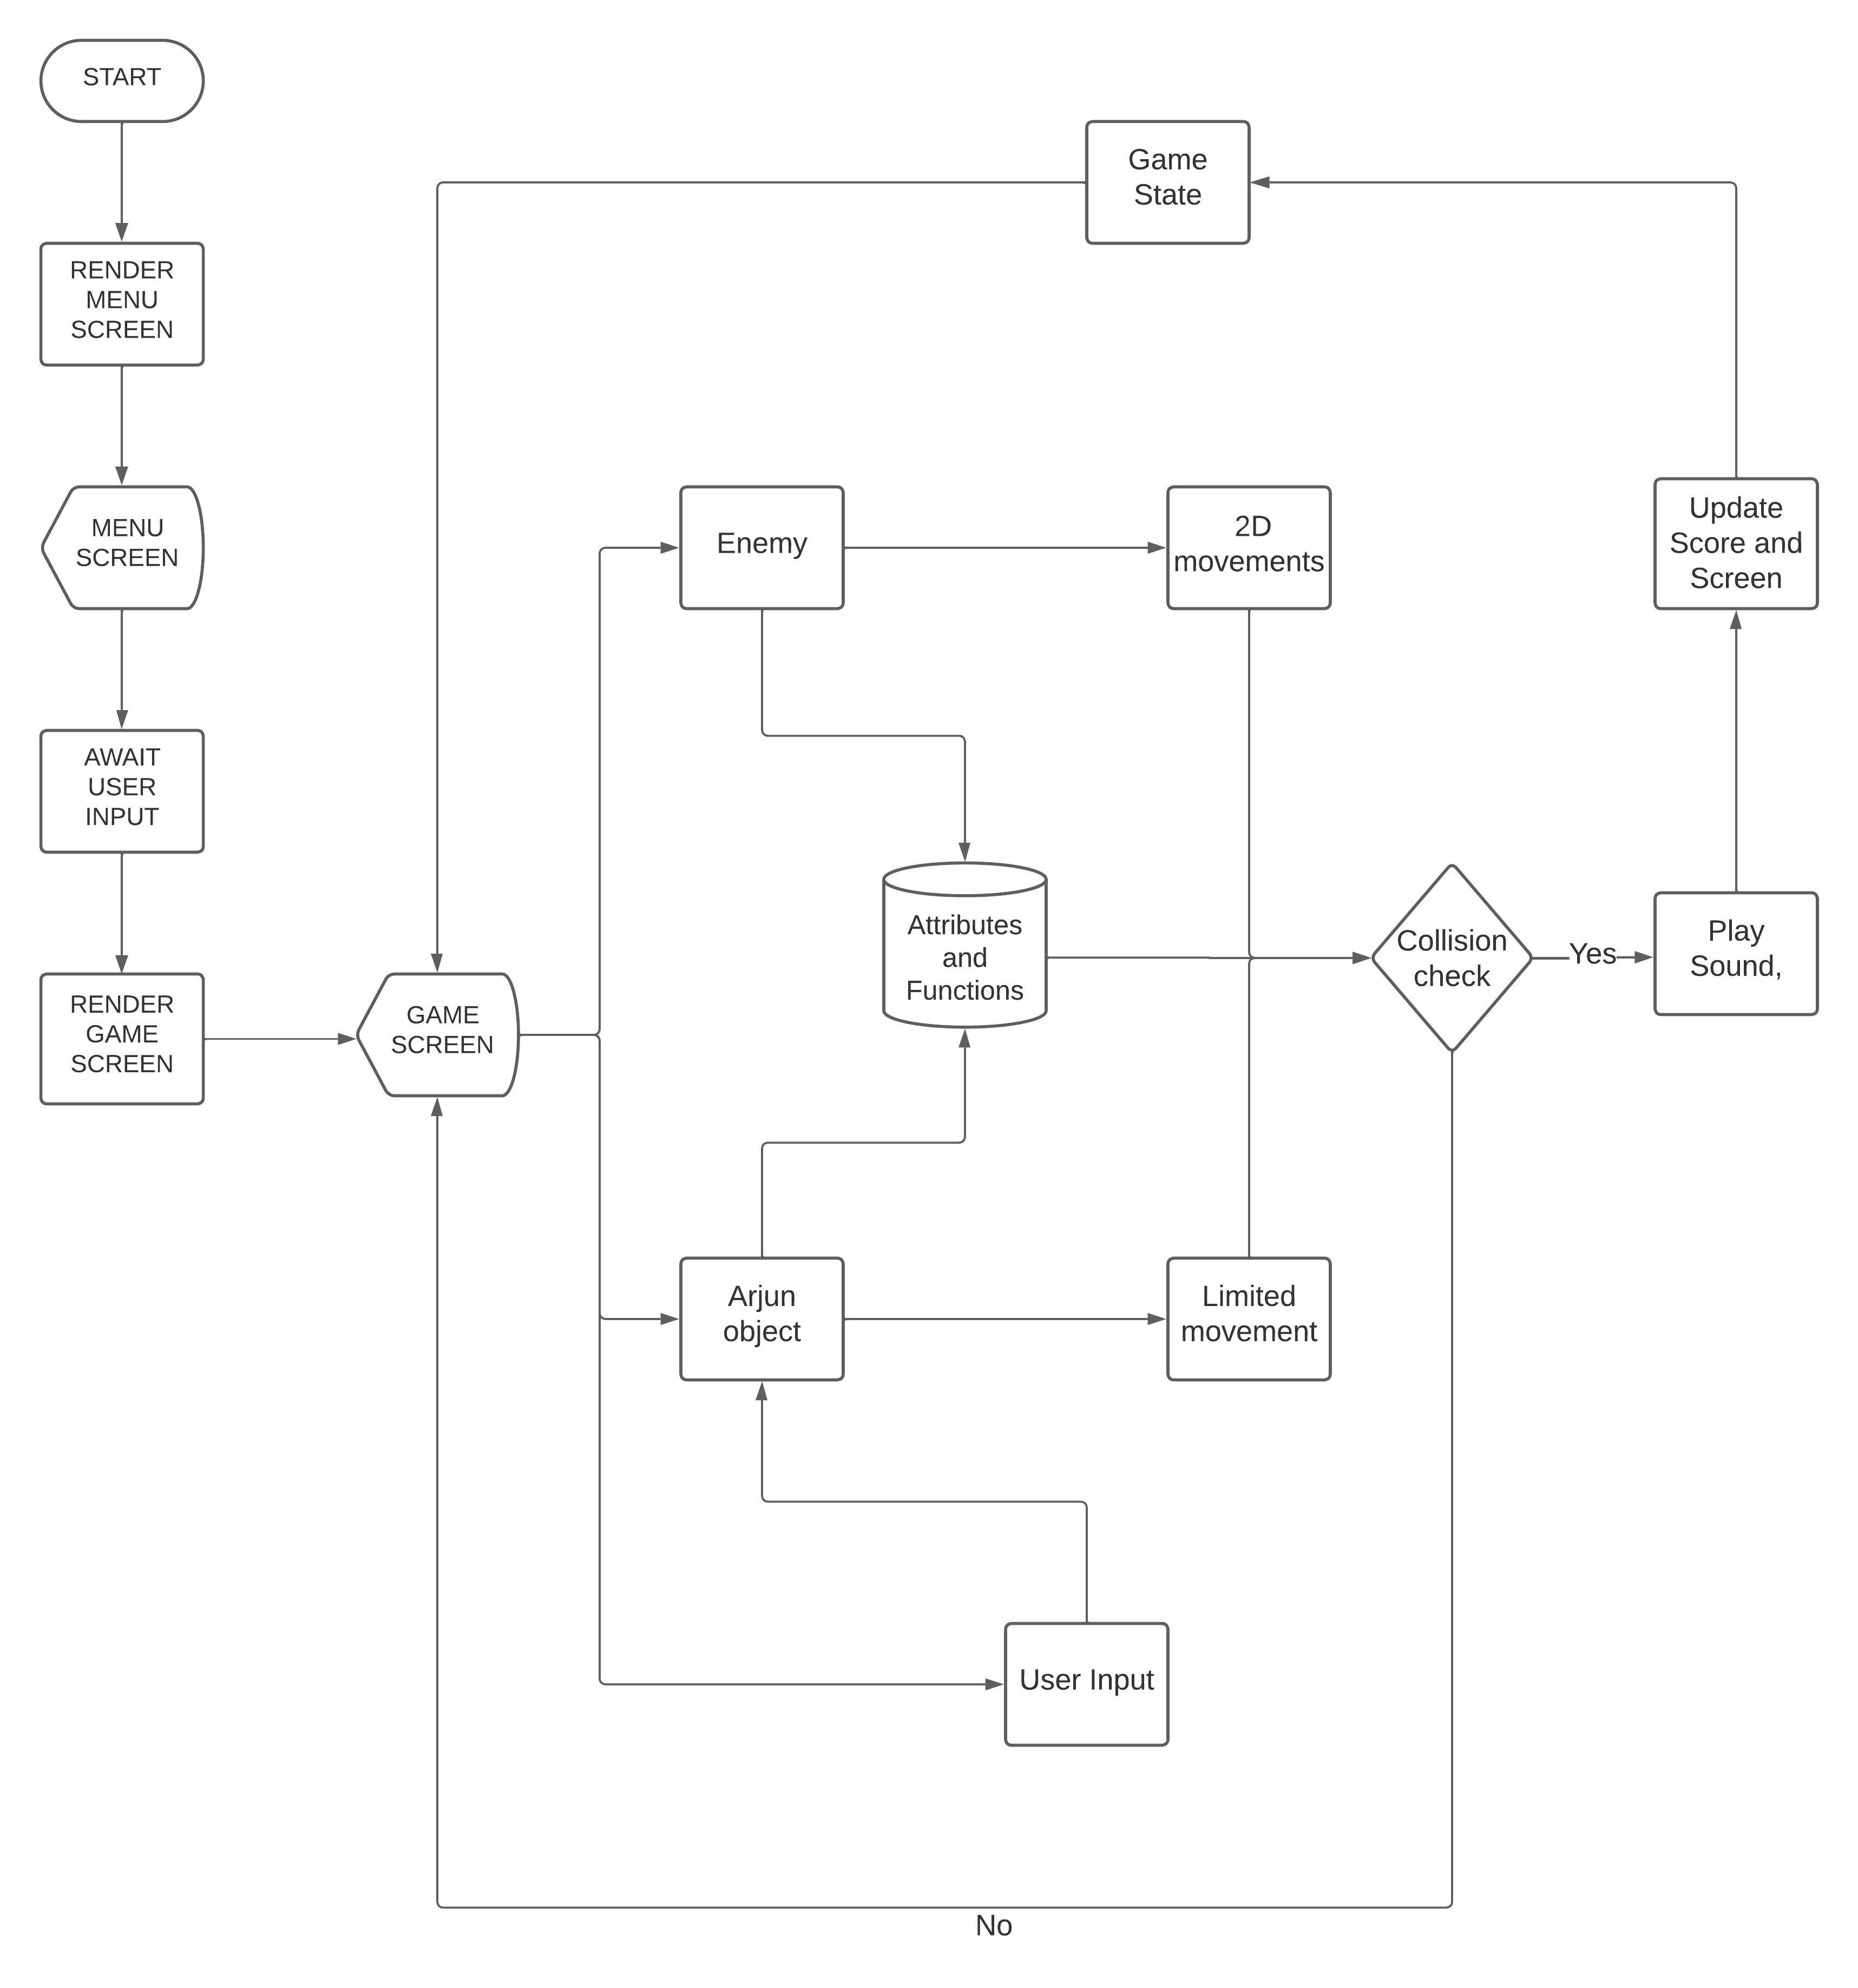
\includegraphics[width = 1.1\textwidth]{sec/pdf/img}

\end{figure}

  	
\section{METHODOLOGY}
To complete our project, we followed the following methods:


	\subsection{Research and Planning} 
	\begin{enumerate}
		\item  Conduct research on various aspects of game development, including features, fundamental requirements, and tools required.
		\item Familiarize ourselves with the necessary libraries and divide the work among the team members.
		\item Develop comprehensive coding guidelines to ensure self-documenting code.
		
	\end{enumerate}
	\subsection{ Algorithm Design }
	\begin{enumerate}
		
		\item Design the algorithm and create a flowchart based on the gathered rules and information. 
		\item Develop a basic prototype for testing purposes, using the console.
		
		
	\end{enumerate}
	
 \subsection{Sources}
	Utilize the following sources as references to support our project:
	\begin{enumerate}
		
		\item Documentation for SFML.
		\item Concepts of object-oriented programming (OOP) and C++ programming from college courses, online references, books, etc.
		
		
	\end{enumerate}
	
	\subsection{ Game Design}
	
	\begin{enumerate}
		
		\item Implement the code using an object-oriented programming (OOP) paradigm. 
		\item Use Simple and Fast Multimedia Library to create build the game.
		\item Choose Visual Studio as our Integrated Development Environment (IDE) and visual c++ as the compiler in the Windows Operating System.
		\item Manage our code using GitHub for version control.
		
	\end{enumerate}
	
 \subsection{Maintenance}
	Regularly maintain the project by following these procedures:
	\begin{enumerate}
		
		\item Corrective maintenance:
		\begin{itemize}
			\item Compile and check specific parts of the code for potential bugs and errors, fixing them as necessary.
		\end{itemize}
		
		\item  Preventive maintenance:
		\begin{itemize}
			
			\item Identify errors and take measures to avoid them during runtime and the development cycle.
			\item Comment and document the source code thoroughly and back it up to prevent potential data loss.
			
			
		\end{itemize}
	\end{enumerate}

	\subsection{Testing and Debugging}
	\begin{enumerate}
		
		\item Develop a minimum viable product sample for testing and debugging purposes.
		\item Conduct frequent testing and debugging to add features and make necessary edits to the project code based on our requirements and capabilities.
		
	\end{enumerate}
	\subsection{ Documentation}
	\begin{enumerate}
		\item Ensure comprehensive documentation of the app, including the addition of copyright licenses.
		\item Ship the completed app with the accompanying documentation.
	\end{enumerate}


\newpage



  		\newpage
\section{PROJECT SCOPE}
Our project involves developing an exciting game based on the character Arjun from Mahabharat. Players will control Arjun and use their mouse to shoot arrows at targets while moving in the game world.

The key aspects of the project scope include:

\begin{enumerate}
	\item User Engagement:
		We aim to create an engaging game that immerses players in the world of Arjun. By providing an enjoyable experience, we hope to entertain players and make them feel connected to the character and the epic.
	
	\item Skill Development:
	The gameplay mechanics, such as arrow shooting and precision aiming, offer players the chance to improve their hand-eye coordination, concentration, and reflexes. These skills can be valuable not just in the game, but also in real-life situations.
	
	\item Cultural Appreciation:
		Our game's theme, inspired by Mahabharat, aims to spark interest and curiosity among players who are fans of the epic or have an interest in Hindu mythology and culture. We want to contribute to cultural appreciation and raise awareness of this rich heritage.
	
	\item Learning and Engagement with Mahabharat:
	 Through the gameplay and accompanying content, we want to provide players with an opportunity to learn more about Arjun and his role in Mahabharat. By delving into the mythology, players can gain insights and develop a deeper understanding of the epic.
	 
	 \item Entertainment Industry Impact: 
	 If our game gains popularity and positive reception, it could have an impact on the entertainment industry. It may inspire similar projects and encourage the exploration of Indian mythological themes in gaming, diversifying the offerings in the industry.
\end{enumerate}


Our project aims to develop an immersive and enjoyable game centered around Arjun from Mahabharat. We want to provide players with an engaging experience, improve their skills, foster cultural appreciation, facilitate learning about Mahabharat, and potentially contribute to the broader landscape of the entertainment industry.

\pagebreak


  	
\section{PROJECT SCHEDULE}
Following is the planned project schedule for our project:
\begin{figure}[h]
	\centering
	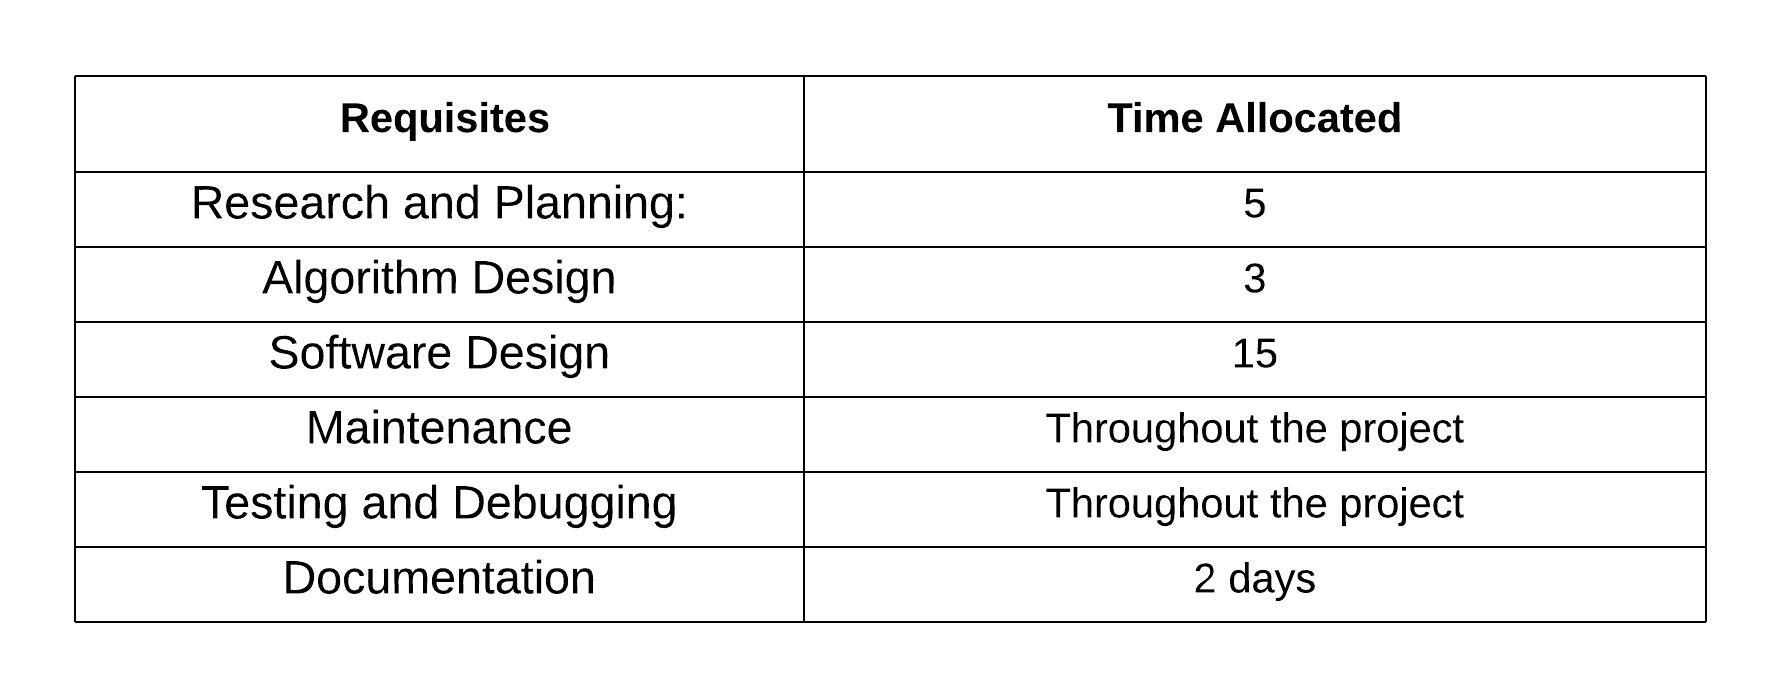
\includegraphics{sec/pdf/schedule1}
\end{figure}


  	
  	
  	
  	
  	
  
  
  
  
	
\end{document}


